\section{Background}\label{sec:background}


\subsection{Representation Schemes}\label{sec:aaaa}

A \emph{representation scheme} for solid modeling is a mapping between a space of mathematical models and a space of symbolic representations, often generated by a formal grammar.
Solid pointsets (i.e., `$r$-sets') are defined~\cite{Requicha:1980:RRS:356827.356833} as compact (bounded and closed) regular and semianalytic subsets of the $d$-space. A large number of representation schemes were defined in the past forty years, including the two main classes of (a) \emph{boundary representations} (`$B$-reps'), where the solid model is represented through a representation of its boundary elements, i.e.~faces, edges and vertices, and (b) \emph{decompositive/enumerative representations}, that are a decomposition of either the object or the embedding space, respectively, into a well-defined \emph{cellular complex}. In particular, a boundary representation provides a cellular decomposition of the object's boundary into \emph{cells} of dimension zero (vertices), one (edges), and two (faces). Medical imaging can be classified as \emph{enumerative representation} of cellular decompositions of organs and tissues of interest, in particular, as subsets \emph{of 3D volume elements} (voxels) from the 3D image. 


\subsection{Linear Algebraic Representation}\label{sec:aaaa}

The \emph{Linear Algebraic Representation} (\textsc{lar})~\cite{Dicarlo:2014:TNL:2543138.2543294} aims to represent the \emph{chain complex}~\cite{TSAS} generated by a piecewise-linear geometric complex embedded either in 2D or in 3D. In few words, it gets a minimal characterization of geometry and topology of a cellular complex, i.e.~the embedding mapping $\mu : C_0 \to \E^d$ of 0-cells (vertices), as well a description of $(d-1)$-cells as subsets of vertices, and is able to return the whole chain complex 
\[ 
C_\bullet = (C_p, \partial_p) := 
C_3 \ 
\substack{
\delta_2 \\
\longleftarrow \\[-1mm]
\longrightarrow \\
\partial_3 
}
\ C_2 \ 
\substack{
\delta_1 \\
\longleftarrow \\[-1mm]
\longrightarrow \\
\partial_2 
}
\ C_1 \ 
\substack{
\delta_0 \\
\longleftarrow \\[-1mm]
\longrightarrow \\
\partial_1 
}
\ C_0 .
\] 
and, in particular, any basis for linear chain spaces $C_p$, and any linear
boundary/coboundary map \(\partial_p\) and
\(\delta_p=\partial_{p+1}^\top\) between them. The domain of \textsc{lar} is the set of chain complexes generated by cell $d$-complexes ($2\leq d\leq 3$). The computer representations of \textsc{lar} are sparse binary matrices to represent both the operators and the chain bases. Note that in algebraic topology a $p$-chain is defined as a linear combination of $p$-cells with scalars from a field. When the scalar coefficients are from $\{-1, 0, +1\}$, a chain may represent \emph{any (oriented) subset of cells} from the cellular complex. 

We may therefore get the $(p-1)$-boundary $\partial_p \gamma_p$ of \emph{any} $p$-chain $\gamma_p$, by multiplication of the coordinate representation $[\partial_p]$ of the boundary operator times the coordinate representation $[\gamma_p]$ of the chain in terms of such scalars, i.e.~by a  matrix-vector product $ [\partial_p] [\gamma_p] $.

It is easy to understand that the \textsc{lar} representation scheme is very expressive, i.e.~that it  has a large domain,  including collections of: line segments, quads, triangles, polygons, meshes;  pixels, voxels, volume images; B-reps, enumerative and decompositive representations of solids. 
In this paper we apply \textsc{lar} methods to computation of boundary representations of solid models from segmentation (labeling) of 3D medical images.

\subsubsection{Construction of $\partial_d$ boundary matrix}

Once fixed an ordering for all the cells (vertices, edges, pixels, and voxels), i.e.~for 0-, 1-, 2-, and 3-elements of a cell partitioning of a 3D image, i.e., once fixed the $p$-bases for linear spaces $C_p$ of $p$-chains $(0\leq p\leq d)$, we call $M_p = (m_{i,j})$ the \emph{characteristic matrix} of the $p$-basis, expressed as subsets of 0-cells, where  we have that $m_{i,j}=1$ iff the $j$-th $0$-cell belongs to the $i$-th $p$-cell, and $m_{i,j}=0$ otherwise.  

Note that, by computing the (sparse) matrix product $(M_{p-1} M_{p}^t) = (n_{i,j})$, with $n_{i,j} = \sum_{k} m_{i,k}m_{k,j}$, we get for each $n_{ij}$ the \emph{number of vertices} shared by $c_{p-1}^i$ and $c_{p}^j$. When this number equates the cardinality of $c_{p-1}^i$, this elementary chain is contained on the boundary of $c_{p}^j$. In a 3D image, with cubic 3-cells and squared 2-cells, everywhere we get $n_{i,j}=4$, we may state $c_{2}^i\subset\partial c_{3}^j$. In this case, by looking in each $j$ column of $M_{2} M_{3}^t = (n_{i,j})$, we have exactly \emph{six rows} where  $n_{i,j} = 4$. 

Finally, consider the linear graded boundary operator $\partial_p : C_p \to C_{p-1}$. As such, it contains by columns the representation of domain basis elements, expressed as linear combination of the basis elements of the range space. Therefore, the operator matrix $[\partial_d]$ is readily obtained by setting $[\partial_d](i,j)=1$ iff $n_{i,j}=4$ and $[\partial_d](i,j)=0$ otherwise.  Of course, it will contain six non-zero elements for column.  It may be worth to remember that every 3-cell (voxel) has exactly six 2-faces. 

It is possible to show that all the interesting relation of incidence/adjacency between cells of different dimensions can be both computed and efficiently queried by pairwise computing some products, with one of terms possibly transposed, of the two boundary and coboundary operator matrices $[\partial_p]$ and $[\delta_p] = [\partial_p^\top] = [\partial_p]^t$. We may also show that such matrices are \emph{very sparse}, with their sparseness growing rapidly with the dimensions (see Section~\ref{sec:block}). The pattern of non-zeros in matrix $[\partial_3]$ corresponding to a brick of shape $(4,4,4)$ is given in Figure~\ref{fig:boundary_matrix_4x4x4}.

\begin{figure}[htbp] %  figure placement: here, top, bottom, or page
   \centering
   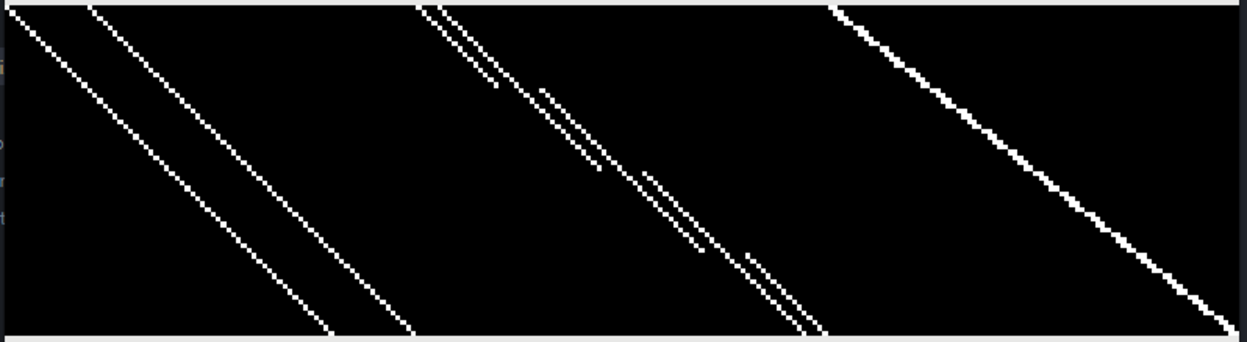
\includegraphics[width=0.75\linewidth]{figs/boundary_matrix_4x4x4.pdf} 
   \caption{A binary image of the coboundary operator  $\delta_2 = \partial^\top : C_2 \to C_3$, built for small 3D images with shape $(4,4,4)$. Note that the number of rows equates the cardinality $4\times 4\times 4 = 64$ of the voxel set; the number of columns is $d\,n\,(1+n)^{d-1} = 3\times 4\times 25 = 300$. Of course, the number of non-zeros per row (cardinality of single voxel facets) is six.}
   \label{fig:boundary_matrix_4x4x4}
\end{figure}

\subsection{Multiindices from Cartesian indices}\label{sec:aaaa}

In order to utilize the topological algebra shortly recalled in this paper, we need to explicitly sort the cells of the various dimensions into linearly ordered sequences, possibly according to the linear order their information is linearly accommodated in computer storage. 

\subsection{Taubin Smoothing}\label{sec:aaaa}



